\documentclass[tikz]{standalone}

\usetikzlibrary{arrows, shapes, positioning}

\begin{document}
    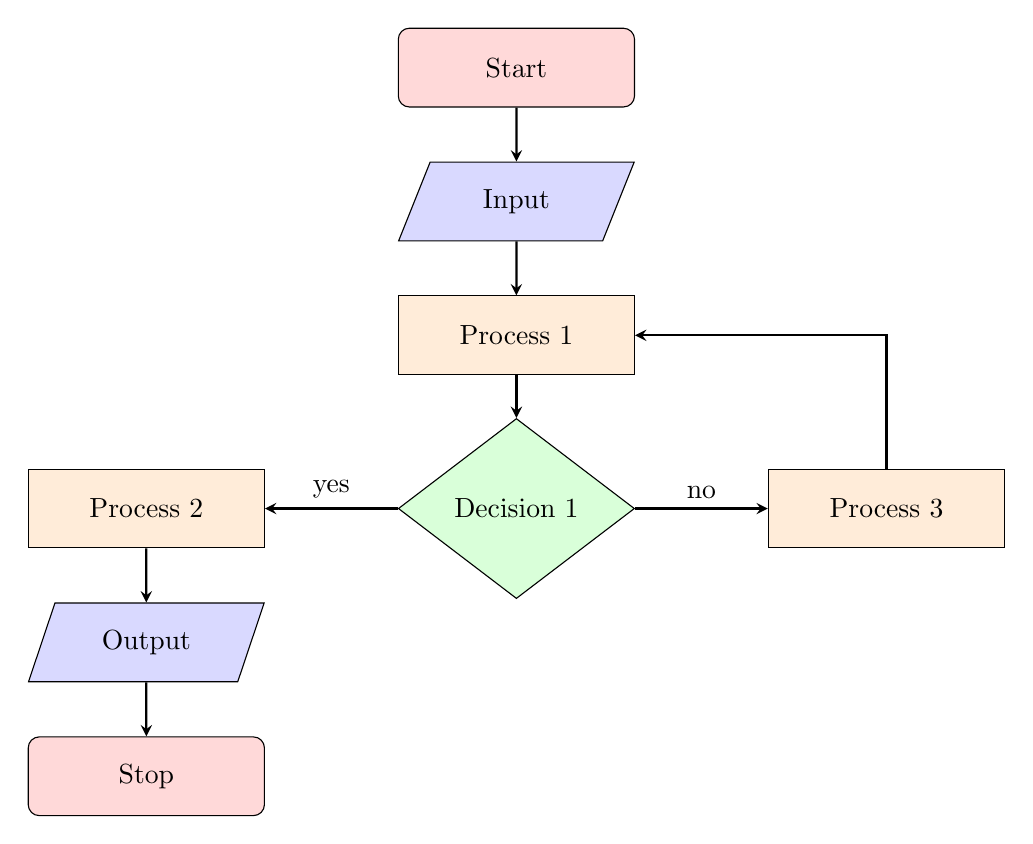
\begin{tikzpicture}[scale=1, node distance=1.7cm]
        \tikzstyle{startstop} = [
    rectangle,
    rounded corners,
    minimum width=3cm,
    minimum height=1cm,
    text centered,
    draw=black,
    fill=red!15
]
\tikzstyle{io} = [
    trapezium,
    trapezium left angle=70,
    trapezium right angle=110,
    minimum width=3cm,
    minimum height=1cm,
    text centered,
    trapezium stretches=true,
    draw=black,
    fill=blue!15
]
\tikzstyle{process} = [
    rectangle,
    minimum width=3cm,
    minimum height=1cm,
    text centered,
    draw=black,
    fill=orange!15
]
\tikzstyle{decision} = [
    diamond,
    minimum width=3cm,
    minimum height=1cm,
    text centered,
    draw=black,
    fill=green!15
]
\tikzstyle{arrow} = [thick, ->, >=stealth]


        \node[startstop] (start) {Start};
        \node[io, below of=start] (input) {Input};
        \node[process, below of=input] (proc1) {Process 1};
        \node[decision, below of=proc1,  yshift=-0.5cm] (dec1) {Decision 1};

        \node[process, left of=dec1, xshift=-3cm] (proc2) {Process 2};
        \node[process, right of=dec1, xshift=3cm] (proc3) {Process 3};

        \node[io, below of=proc2] (output) {Output};
        \node[startstop, below of=output] (stop) {Stop};

        \draw[arrow] (start) -- (input);
        \draw[arrow] (input) -- (proc1);
        \draw[arrow] (proc1) -- (dec1);
        \draw[arrow] (dec1) -- node[above] {yes} (proc2);
        \draw[arrow] (dec1) -- node[above] {no} (proc3);
        \draw[arrow] (proc3) |- (proc1);
        \draw[arrow] (proc2) -- (output);
        \draw[arrow] (output) -- (stop);
    \end{tikzpicture}
\end{document}
